%  Copyright 2020-2026 Robert Bosch GmbH
%
%  Licensed under the Apache License, Version 2.0 (the "License");
%  you may not use this file except in compliance with the License.
%  You may obtain a copy of the License at
%
%      http://www.apache.org/licenses/LICENSE-2.0
%
%  Unless required by applicable law or agreed to in writing, software
%  distributed under the License is distributed on an "AS IS" BASIS,
%  WITHOUT WARRANTIES OR CONDITIONS OF ANY KIND, either express or implied.
%  See the License for the specific language governing permissions and
%  limitations under the License.

\section{Configuration}
\begin{boxhint}{Pre-condition}
Ensure the \textbf{GitHub Copilot} Extensions are installed and you are signed
in with your GitHub account.

Please refer to the chapter \hyperref[chap:copilot]{GitHub Copilot Extension}
for detailed installation and sign-in instructions.

\end{boxhint}

Steps to configure Roo Code Extension to use GitHub Copilot:
\begin{enumerate}
   \item Open \textbf{VSCodium For RobotFramework}.
   \item Click the \textbf{Roo Code icon} in the Activity Bar.
   \item Select \textbf{Use another provider} option at Welcome screen of extension (First time use).

         Or click the \textbf{Settings (gear icon)} at the top of the Roo Code panel (Already configured).
   \item In the \textbf{API Provider} option, select \textbf{VS Code LM API}
      as the provider.
   \item Choose the available model within the dropdown menu.
   \item Click \textbf{Done}.
\end{enumerate}

Refer to the images below for guidance:

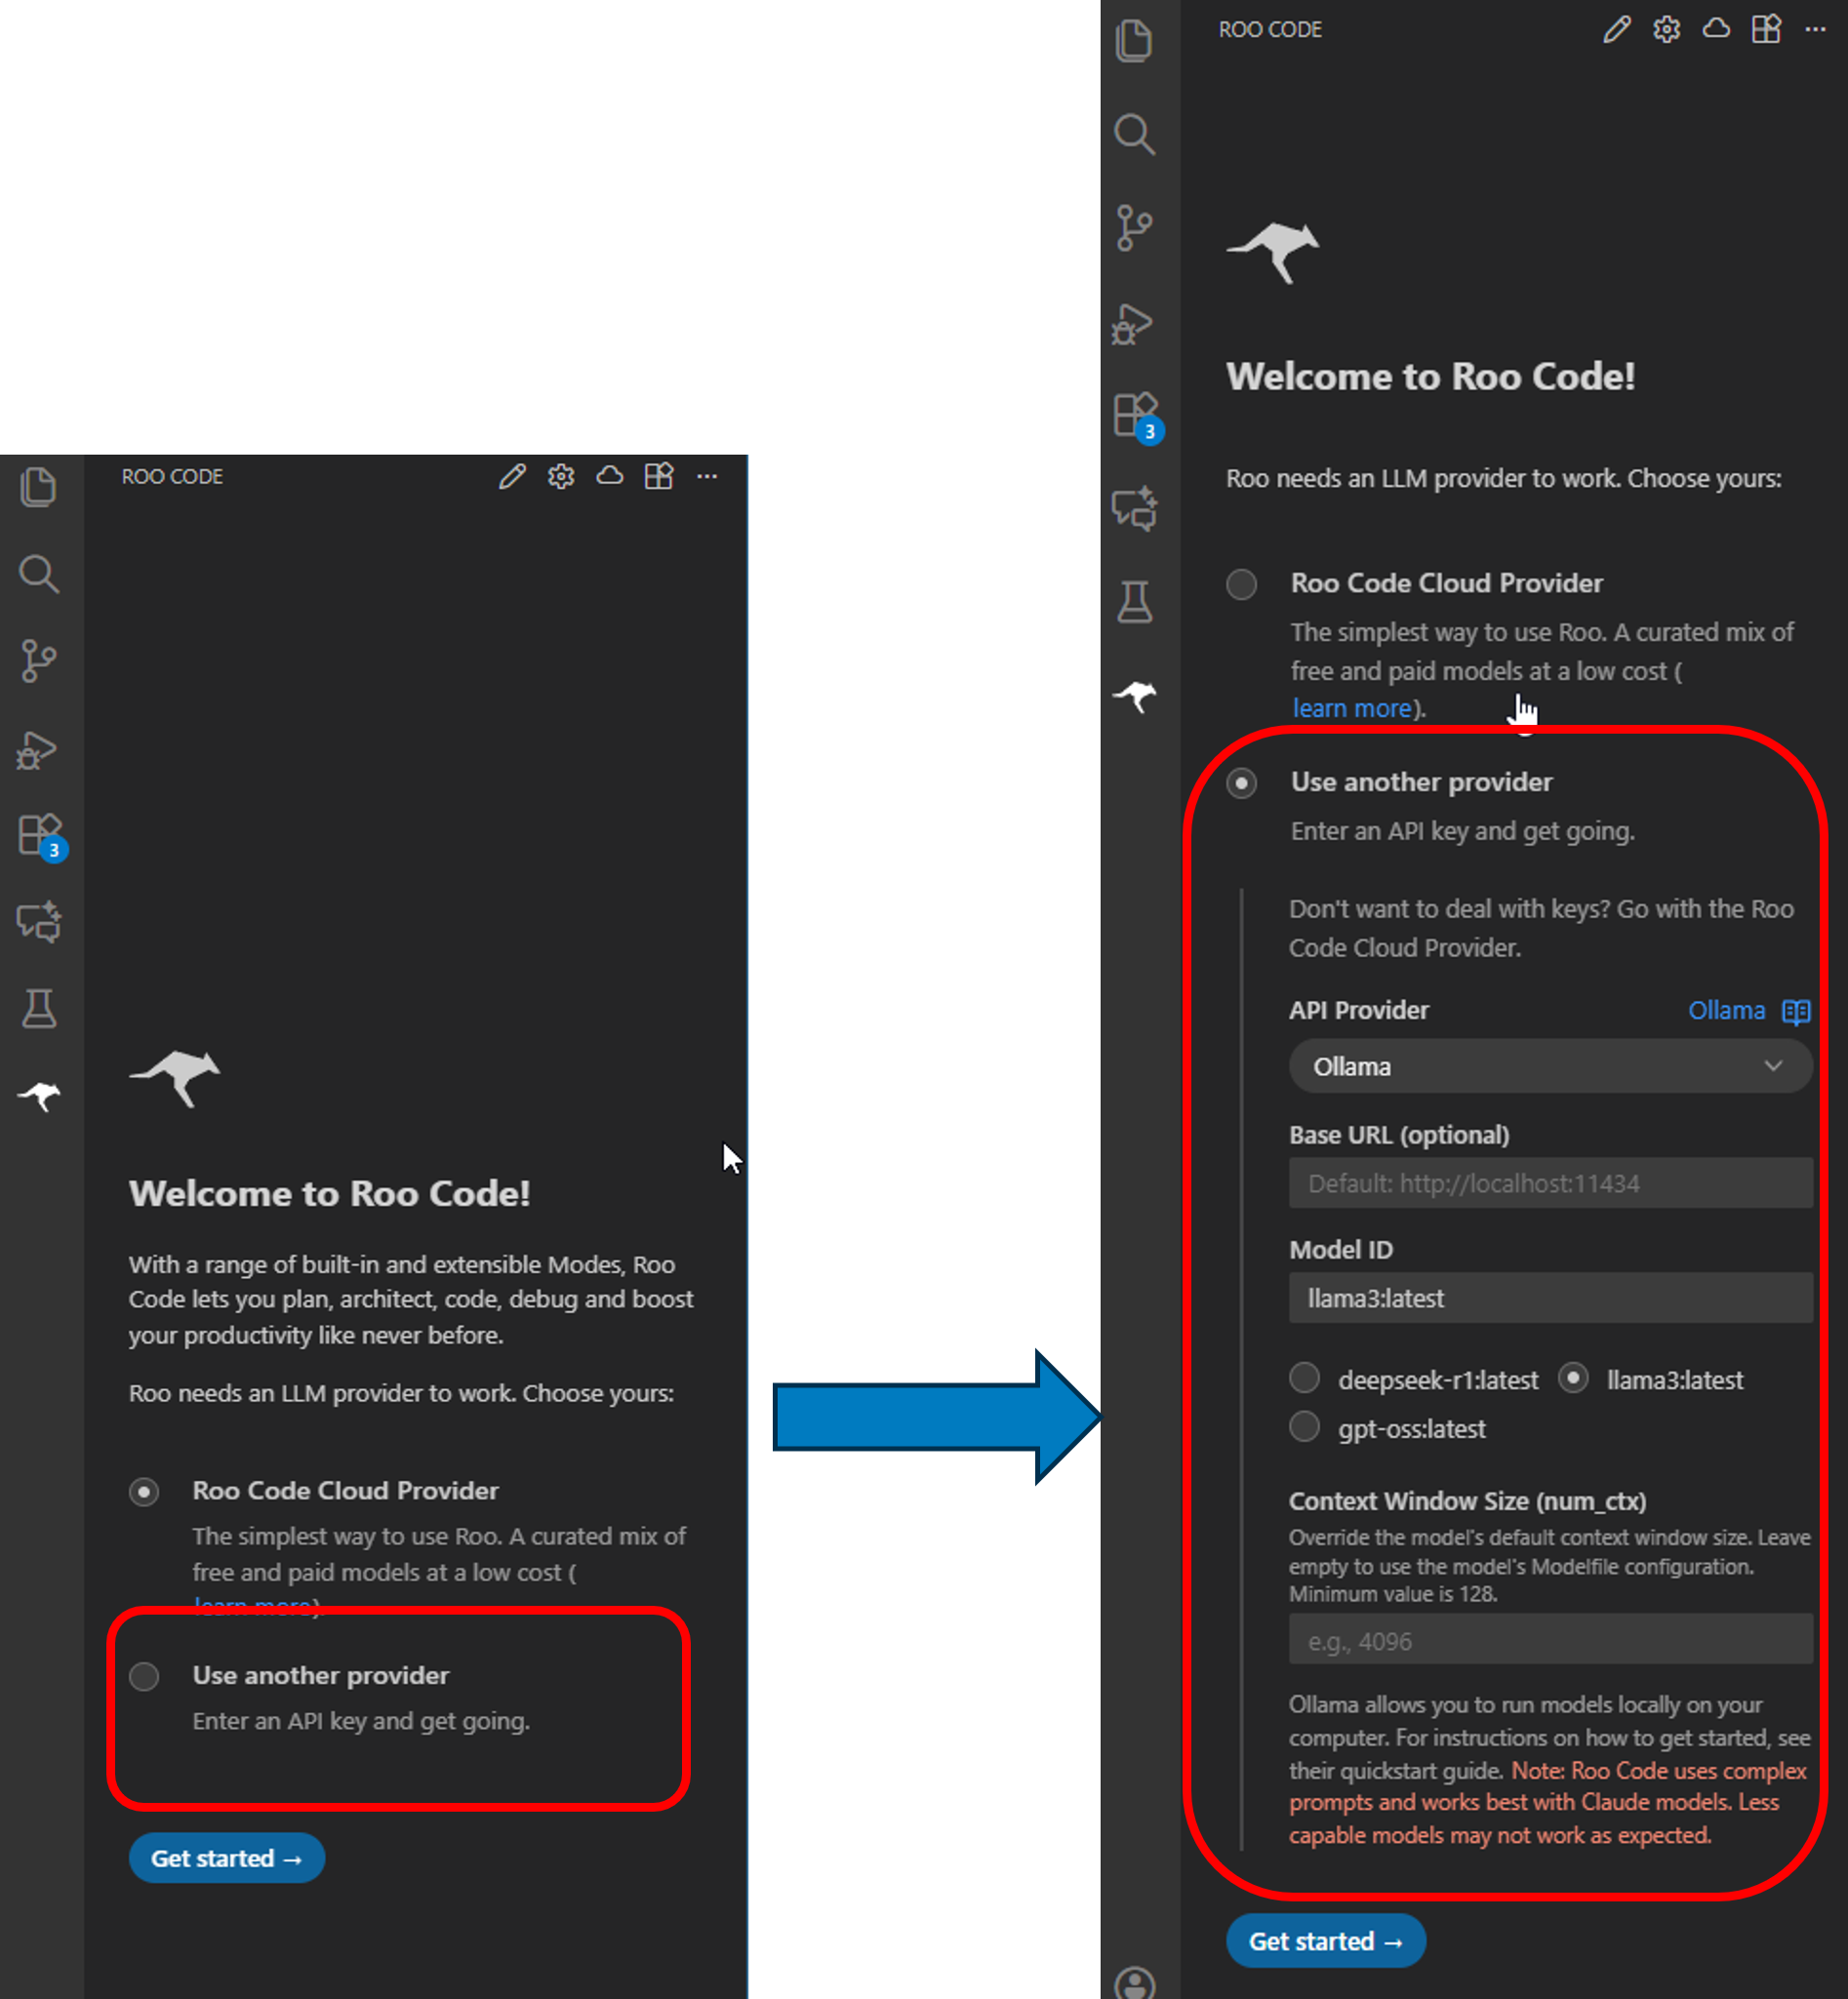
\includegraphics{./include/graphics/roocode/RooCodeUseLLMProviders.png}

\includegraphics{./include/graphics/roocode/GitHubCopilotLLM.png}
